% !TeX program = lualatex
% Author         : Pedro Ferreira (up201806093@up.pt)
% Version        : 1.0
% Created on     : 12.08.2022
% Last Edited on : 14.08.2022

% Adapted from HSRM theme by Benjamin Weiss
% Copyright      : Copyright (c) 2013-2014 by Benjamin Weiss. All rights reserved.
% License        : This file may be distributed and/or modified under the
%                  GNU Public License.
% Description    : HSRM beamer theme demonstration. Also includes a short 
%                  Tutorial regarding the beamer class.

\documentclass[compress,aspectratio=169]{beamer}

%--------------------------------------------------------------------------
% Custom commands
%--------------------------------------------------------------------------
\newcommand\insertcourse{}  % Empty by default.
\newcommand\course[1]{\renewcommand\insertcourse{#1}}

%--------------------------------------------------------------------------
% Common packages
%--------------------------------------------------------------------------
\usepackage[british]{babel}
\usepackage{graphicx}
\usepackage{multicol}

% Advanced table functions
\usepackage{tabularx,ragged2e}
\usepackage{booktabs}
% Listings extension
\usepackage{listings}
\lstset{ %
language=[LaTeX]TeX,
basicstyle=\normalsize\ttfamily,
keywordstyle=,
numbers=left,
numberstyle=\tiny\ttfamily,
stepnumber=1,
showspaces=false,
showstringspaces=false,
showtabs=false,
breaklines=true,
frame=tb,
framerule=0.5pt,
tabsize=4,
framexleftmargin=0.5em,
framexrightmargin=0.5em,
xleftmargin=0.5em,
xrightmargin=0.5em
}

%--------------------------------------------------------------------------
% Load theme
%--------------------------------------------------------------------------
\usepackage[footline]{sleektheme/beamerthemesleek}
\usetheme{sleek}

\usepackage{sleektheme/dtklogos} % must be loaded after theme
\usepackage{tikz}
\usetikzlibrary{mindmap,backgrounds}

%--------------------------------------------------------------------------
% General presentation settings
%--------------------------------------------------------------------------
\title{Sleek Beamer Theme}
\subtitle{Demonstration and short introduction to beamer}
\date{Last Update: \today}
\author{Pedro Ferreira}
\institute{DEMEC\\ {\Medium FEUP}}
\course{Beamer Themes}
\hypersetup{
	pdftitle={Sleek Beamer Theme},
	pdfsubject={Latex Beamer},
	pdfauthor={Pedro Paulo Carneiro Ferreira},
	pdfkeywords={Latex,Beamer}}

% The titlepage background opacity can be tweaked in the file title_page.dtx

%--------------------------------------------------------------------------
% Notes settings
%--------------------------------------------------------------------------
\setbeameroption{show notes}

\begin{document}
%--------------------------------------------------------------------------
% Titlepage
%--------------------------------------------------------------------------

\maketitle


%--------------------------------------------------------------------------
% Table of contents
%--------------------------------------------------------------------------
\section*{Structure}
\begin{frame}{Structure}
	% hideallsubsections is recommended for longer presentations
	\tableofcontents[hideallsubsections]
\end{frame}

%--------------------------------------------------------------------------
% Content
%--------------------------------------------------------------------------
\section{Introduction}

\begin{frame}{What is Beamer?}
	The beamer classes for \LaTeX\ are used to create presentations that are to be shown with a beamer. The text typesetting system creates PDF files that can be shown by a large number of programmes.
	
	The present theme was adapetd from HSRM theme by Benjamin Weiss and it makes the creation of slides (assuming basic knowledge of \LaTeX\ ) child's play.
\end{frame}

\begin{frame}{System requirements}
	In order to successfully create presentations with this theme, the following requirements must be met by the system:
	\begin{itemize}
		\item LuaLaTeX must be used to typeset the slides.
		\item Besides some standard packages, the packages \texttt{beamer}, \texttt{pgf} and \texttt{xcolor} must be installed.
		\item The fonts \quoted{Flama-Light}, \quoted{Flama-Book} and \quoted{Flama-Medium} should be installed. Alternative: \quoted{Arial}\\\url{http://www.felicianotypefoundry.com/}
	\end{itemize}
\end{frame}

\section{Tutorial}
\begin{frame}[containsverbatim]{Basic structure of the document}
The basic structure is simple:
\begin{lstlisting}
\documentclass[compress]{beamer}
% Theme
\usetheme{sleek}
% General presentation settings 
\title{Presentation title}
\subtitle{Subtitle of the presentation}
\author{Your name}
\institute{Study area \\ {\Medium FEUP}}
\begin{document}
%Slides
\end{document}
\end{lstlisting}
\end{frame}

\begin{frame}{Theme options}
To customise the presentation, the following options can be specified when loading the theme package, in the options field, \texttt{\textbackslash usepackage[options]\{package\}}.
\begin{table}[]
	\begin{tabularx}{\linewidth}{l>{\raggedright}X}
		\toprule
		\textbf{Option} & \textbf{Effect} \tabularnewline
		\midrule
		\texttt{noflama} & If you do not want the Flama font you can switch to the Arial font with this option. \tabularnewline
		\texttt{noserifmath} & Formulas are also set sans serif. \tabularnewline
		\texttt{nosectionpages} & The section introduction pages will be hidden.\tabularnewline
		\texttt{footline} & Footline with author, course and slide number. \tabularnewline
		\bottomrule
	\end{tabularx}
	\label{tab:options}
\end{table}
\end{frame}

\begin{frame}{Primary colours}									
All colours predefined are listed below and in the following slides. You may add more using the same code structure as in the \texttt{colors.tex} file.


\begin{multicols}{2}

\setbeamercolor{sleekmaincolorDemo}{fg=maincolor,bg=white}
\begin{beamercolorbox}[wd=\linewidth,ht=2ex,dp=0.7ex]{sleekmaincolorDemo}
	\texttt{maincolor}
\end{beamercolorbox}
\setbeamercolor{sleekRedDemo}{fg=sleekRed,bg=white}
\begin{beamercolorbox}[wd=\linewidth,ht=2ex,dp=0.7ex]{sleekRedDemo}
	\texttt{sleekRed}
\end{beamercolorbox}
\setbeamercolor{sleekRedDarkDemo}{fg=sleekRedDark,bg=white}
\begin{beamercolorbox}[wd=\linewidth,ht=2ex,dp=0.7ex]{sleekRedDarkDemo}
	\texttt{sleekRedDark}
\end{beamercolorbox}
\setbeamercolor{sleekWarmGreyDarkDemo}{fg=sleekWarmGreyDark,bg=white}
\begin{beamercolorbox}[wd=\linewidth,ht=2ex,dp=0.7ex]{sleekWarmGreyDarkDemo}
	\texttt{sleekWarmGreyDark}
\end{beamercolorbox}
\setbeamercolor{sleekWarmGreyLightDemo}{fg=sleekWarmGreyLight,bg=white}
\begin{beamercolorbox}[wd=\linewidth,ht=2ex,dp=0.7ex]{sleekWarmGreyLightDemo}
	\texttt{sleekWarmGreyLight}
\end{beamercolorbox}
\setbeamercolor{sleekLightGreyDemo}{fg=sleekLightGrey,bg=white}
\begin{beamercolorbox}[wd=\linewidth,ht=2ex,dp=0.7ex]{sleekLightGreyDemo}
	\texttt{sleekLightGrey}
\end{beamercolorbox}

\setbeamercolor{sleekmaincolorDemoBg}{fg=white,bg=maincolor}
\begin{beamercolorbox}[wd=\linewidth,ht=2ex,leftskip=.5ex,dp=0.7ex]{sleekmaincolorDemoBg}
	\texttt{maincolor}
\end{beamercolorbox}
\setbeamercolor{sleekRedDemoBg}{fg=white,bg=sleekRed}
\begin{beamercolorbox}[wd=\linewidth,ht=2ex,leftskip=.5ex,dp=0.7ex]{sleekRedDemoBg}
	\texttt{sleekRed}
\end{beamercolorbox}
\setbeamercolor{sleekRedDarkDemoBg}{fg=white,bg=sleekRedDark}
\begin{beamercolorbox}[wd=\linewidth,ht=2ex,leftskip=.5ex,dp=0.7ex]{sleekRedDarkDemoBg}
	\texttt{sleekRedDark}
\end{beamercolorbox}
\setbeamercolor{sleekWarmGreyDarkDemo}{fg=white,bg=sleekWarmGreyDark}
\begin{beamercolorbox}[wd=\linewidth,ht=2ex,leftskip=.5ex,dp=0.7ex]{sleekWarmGreyDarkDemo}
	\texttt{sleekWarmGreyDark}
\end{beamercolorbox}
\setbeamercolor{sleekWarmGreyLightDemo}{fg=white,bg=sleekWarmGreyLight}
\begin{beamercolorbox}[wd=\linewidth,ht=2ex,leftskip=.5ex,dp=0.7ex]{sleekWarmGreyLightDemo}
	\texttt{sleekWarmGreyLight}
\end{beamercolorbox}
\setbeamercolor{sleekLightGreyDemo}{fg=white,bg=sleekLightGrey}
\begin{beamercolorbox}[wd=\linewidth,ht=2ex,leftskip=.5ex,dp=0.7ex]{sleekLightGreyDemo}
	\texttt{sleekLightGrey}
\end{beamercolorbox}

\end{multicols}

\end{frame}

\begin{frame}{Secondary colours}
\begin{multicols}{2}
\setbeamercolor{sleekSec1Demo}{fg=sleekSec1,bg=white}
\begin{beamercolorbox}[wd=\linewidth,ht=2ex,dp=0.7ex]{sleekSec1Demo}
	\texttt{sleekSec1}
\end{beamercolorbox}
\setbeamercolor{sleekSec1DarkDemo}{fg=sleekSec1Dark,bg=white}
\begin{beamercolorbox}[wd=\linewidth,ht=2ex,dp=0.7ex]{sleekSec1DarkDemo}
	\texttt{sleekSec1Dark}
\end{beamercolorbox}
\setbeamercolor{sleekSec1CompDemo}{fg=sleekSec1Comp,bg=white}
\begin{beamercolorbox}[wd=\linewidth,ht=2ex,dp=0.7ex]{sleekSec1CompDemo}
	\texttt{sleekSec1Comp}
\end{beamercolorbox}
\setbeamercolor{sleekSec1CompDarkDemo}{fg=sleekSec1CompDark,bg=white}
\begin{beamercolorbox}[wd=\linewidth,ht=2ex,dp=0.7ex]{sleekSec1CompDarkDemo}
	\texttt{sleekSec1CompDark}
\end{beamercolorbox}
\setbeamercolor{sleekSec2Demo}{fg=sleekSec2,bg=white}
\begin{beamercolorbox}[wd=\linewidth,ht=2ex,dp=0.7ex]{sleekSec2Demo}
	\texttt{sleekSec2}
\end{beamercolorbox}
\setbeamercolor{sleekSec2DarkDemo}{fg=sleekSec2Dark,bg=white}
\begin{beamercolorbox}[wd=\linewidth,ht=2ex,dp=0.7ex]{sleekSec2DarkDemo}
	\texttt{sleekSec2Dark}
\end{beamercolorbox}
\setbeamercolor{sleekSec2CompDemo}{fg=sleekSec2Comp,bg=white}
\begin{beamercolorbox}[wd=\linewidth,ht=2ex,dp=0.7ex]{sleekSec2CompDemo}
	\texttt{sleekSec2Comp}
\end{beamercolorbox}
\setbeamercolor{sleekSec2CompDarkDemo}{fg=sleekSec2CompDark,bg=white}
\begin{beamercolorbox}[wd=\linewidth,ht=2ex,dp=0.7ex]{sleekSec2CompDarkDemo}
	\texttt{sleekSec2CompDark}
\end{beamercolorbox}

%\setbeamercolor{sleekSec3Demo}{fg=sleekSec3,bg=white}
%\begin{beamercolorbox}[wd=\linewidth,ht=2ex,dp=0.7ex]{sleekSec3Demo}
%	\texttt{sleekSec3}
%\end{beamercolorbox}
%\setbeamercolor{sleekSec3DarkDemo}{fg=sleekSec3Dark,bg=white}
%\begin{beamercolorbox}[wd=\linewidth,ht=2ex,dp=0.7ex]{sleekSec3DarkDemo}
%	\texttt{sleekSec3Dark}
%\end{beamercolorbox}
%\setbeamercolor{sleekSec3CompDemo}{fg=sleekSec3Comp,bg=white}
%\begin{beamercolorbox}[wd=\linewidth,ht=2ex,dp=0.7ex]{sleekSec3CompDemo}
%	\texttt{sleekSec3Comp}
%\end{beamercolorbox}
%\setbeamercolor{sleekSec3CompDarkDemo}{fg=sleekSec3CompDark,bg=white}
%\begin{beamercolorbox}[wd=\linewidth,ht=2ex,dp=0.7ex]{sleekSec3CompDarkDemo}
%	\texttt{sleekSec3CompDark}
%\end{beamercolorbox}

\setbeamercolor{sleekSec1DemoBg}{fg=white,bg=sleekSec1}
\begin{beamercolorbox}[wd=\linewidth,ht=2ex,leftskip=.5ex,dp=0.7ex]{sleekSec1DemoBg}
	\texttt{sleekSec1}
\end{beamercolorbox}
\setbeamercolor{sleekSec1DarkDemoBg}{fg=white,bg=sleekSec1Dark}
\begin{beamercolorbox}[wd=\linewidth,ht=2ex,leftskip=.5ex,dp=0.7ex]{sleekSec1DarkDemoBg}
	\texttt{sleekSec1Dark}
\end{beamercolorbox}
\setbeamercolor{sleekSec1CompDemoBg}{fg=white,bg=sleekSec1Comp}
\begin{beamercolorbox}[wd=\linewidth,ht=2ex,leftskip=.5ex,dp=0.7ex]{sleekSec1CompDemoBg}
	\texttt{sleekSec1Comp}
\end{beamercolorbox}
\setbeamercolor{sleekSec1CompDarkDemoBg}{fg=white,bg=sleekSec1CompDark}
\begin{beamercolorbox}[wd=\linewidth,ht=2ex,leftskip=.5ex,dp=0.7ex]{sleekSec1CompDarkDemoBg}
	\texttt{sleekSec1CompDark}
\end{beamercolorbox}

\setbeamercolor{sleekSec2DemoBg}{fg=white,bg=sleekSec2}
\begin{beamercolorbox}[wd=\linewidth,ht=2ex,leftskip=.5ex,dp=0.7ex]{sleekSec2DemoBg}
	\texttt{sleekSec2}
\end{beamercolorbox}
\setbeamercolor{sleekSec2DarkDemoBg}{fg=white,bg=sleekSec2Dark}
\begin{beamercolorbox}[wd=\linewidth,ht=2ex,leftskip=.5ex,dp=0.7ex]{sleekSec2DarkDemoBg}
	\texttt{sleekSec2Dark}
\end{beamercolorbox}
\setbeamercolor{sleekSec2CompDemoBg}{fg=white,bg=sleekSec2Comp}
\begin{beamercolorbox}[wd=\linewidth,ht=2ex,leftskip=.5ex,dp=0.7ex]{sleekSec2CompDemoBg}
	\texttt{sleekSec2Comp}
\end{beamercolorbox}
\setbeamercolor{sleekSec2CompDarkDemoBg}{fg=white,bg=sleekSec2CompDark}
\begin{beamercolorbox}[wd=\linewidth,ht=2ex,leftskip=.5ex,dp=0.7ex]{sleekSec2CompDarkDemoBg}
	\texttt{sleekSec2CompDark}
\end{beamercolorbox}

%\setbeamercolor{sleekSec3Demo}{fg=white,bg=sleekSec3}
%\begin{beamercolorbox}[wd=\linewidth,ht=2ex,leftskip=.5ex,dp=0.7ex]{sleekSec3Demo}
%	\texttt{sleekSec3}
%\end{beamercolorbox}
%\setbeamercolor{sleekSec3DarkDemo}{fg=white,bg=sleekSec3Dark}
%\begin{beamercolorbox}[wd=\linewidth,ht=2ex,leftskip=.5ex,dp=0.7ex]{sleekSec3DarkDemo}
%	\texttt{sleekSec3Dark}
%\end{beamercolorbox}
%\setbeamercolor{sleekSec3CompDemo}{fg=white,bg=sleekSec3Comp}
%\begin{beamercolorbox}[wd=\linewidth,ht=2ex,leftskip=.5ex,dp=0.7ex]{sleekSec3CompDemo}
%	\texttt{sleekSec3Comp}
%\end{beamercolorbox}
%\setbeamercolor{sleekSec3CompDarkDemo}{fg=white,bg=sleekSec3CompDark}
%\begin{beamercolorbox}[wd=\linewidth,ht=2ex,leftskip=.5ex,dp=0.7ex]{sleekSec3CompDarkDemo}
%	\texttt{sleekSec3CompDark}
%\end{beamercolorbox}
\end{multicols}
\end{frame}

\begin{frame}{Secondary colours}
	\begin{multicols}{2}
		\setbeamercolor{sleekSec3Demo}{fg=sleekSec3,bg=white}
		\begin{beamercolorbox}[wd=\linewidth,ht=2ex,dp=0.7ex]{sleekSec3Demo}
			\texttt{sleekSec3}
		\end{beamercolorbox}
		\setbeamercolor{sleekSec3DarkDemo}{fg=sleekSec3Dark,bg=white}
		\begin{beamercolorbox}[wd=\linewidth,ht=2ex,dp=0.7ex]{sleekSec3DarkDemo}
			\texttt{sleekSec3Dark}
		\end{beamercolorbox}
		\setbeamercolor{sleekSec3CompDemo}{fg=sleekSec3Comp,bg=white}
		\begin{beamercolorbox}[wd=\linewidth,ht=2ex,dp=0.7ex]{sleekSec3CompDemo}
			\texttt{sleekSec3Comp}
		\end{beamercolorbox}
		\setbeamercolor{sleekSec3CompDarkDemo}{fg=sleekSec3CompDark,bg=white}
		\begin{beamercolorbox}[wd=\linewidth,ht=2ex,dp=0.7ex]{sleekSec3CompDarkDemo}
			\texttt{sleekSec3CompDark}
		\end{beamercolorbox}
	
		\setbeamercolor{sleekSec3Demo}{fg=white,bg=sleekSec3}
		\begin{beamercolorbox}[wd=\linewidth,ht=2ex,leftskip=.5ex,dp=0.7ex]{sleekSec3Demo}
			\texttt{sleekSec3}
		\end{beamercolorbox}
		\setbeamercolor{sleekSec3DarkDemo}{fg=white,bg=sleekSec3Dark}
		\begin{beamercolorbox}[wd=\linewidth,ht=2ex,leftskip=.5ex,dp=0.7ex]{sleekSec3DarkDemo}
			\texttt{sleekSec3Dark}
		\end{beamercolorbox}
		\setbeamercolor{sleekSec3CompDemo}{fg=white,bg=sleekSec3Comp}
		\begin{beamercolorbox}[wd=\linewidth,ht=2ex,leftskip=.5ex,dp=0.7ex]{sleekSec3CompDemo}
			\texttt{sleekSec3Comp}
		\end{beamercolorbox}
		\setbeamercolor{sleekSec3CompDarkDemo}{fg=white,bg=sleekSec3CompDark}
		\begin{beamercolorbox}[wd=\linewidth,ht=2ex,leftskip=.5ex,dp=0.7ex]{sleekSec3CompDarkDemo}
			\texttt{sleekSec3CompDark}
		\end{beamercolorbox}
	\end{multicols}
\end{frame}

\begin{frame}[containsverbatim]{slide structure}
Structure in Beamer is the same as in \LaTeX\ using \lstinline!section!, \lstinline!subsection!, etc. For slides the \lstinline!frame! environment is defined.

The slide title can be passed directly to the \lstinline!frame! environment or set within the environment using \lstinline!\frametitle{slide title}!
\begin{lstlisting}
\section{My Section}
\subsection{My Subsection}
\begin{frame}
\frametitle{slide title}
% slide content
\end{frame}
\end{lstlisting}
\end{frame}

\begin{frame}[containsverbatim]{title page and table of contents}
The title page is created with 
\begin{lstlisting}
\maketitle
\end{lstlisting}
And the table of contents with
\begin{lstlisting}
\begin{frame}{outline}
	\tableofcontents[hideallsubsections]
\end{frame}
\end{lstlisting}
The option \lstinline!hideallsubsections! is useful for longer presentations to keep the table of contents compact.
\end{frame}

\subsection{Enumerations}
\begin{frame}[containsverbatim]{enumerations}
Enumerations are possible with the \lstinline!enumerate! and the \lstinline!itemize! environment.
\begin{enumerate}
	\item Item 1
	\begin{enumerate}
		\item Nested item
	\end{enumerate}
	\item Item 2
	\begin{itemize}
		\item Point 1
		\item Point 2
	\end{itemize}
	\item Item 3
\end{enumerate}
\end{frame}

\begin{frame}{Enumerations with timings}
	\only<1>{A list may be presented showing each bullet or item one by one. To achieve this result please see the source code for this frame.}
	\begin{multicols}{2}
	\begin{itemize}
		\item<1-> Visible from the 1st slide
		\item<2-> Visible from the 2nd slide
		\item<3-> Visible from the 3rd slide
	\end{itemize}
	\columnbreak
	\setbeamercovered{transparent} % must be placed before \begin{document}
	\begin{itemize}[{<+->}] % This is another way to time the different items, instead of defining them one by one
		\item Visible from the 1st slide
		\item Visible from the 2nd slide
		\item Visible from the 3rd slide
	\end{itemize}
	\end{multicols}
	\only<2>{The standard display style is the one on the left, if you want to see the upcoming items (right column style) just add the command \texttt{\textbackslash setbeamercovered\{transparent\}} before the beginning of the document.}
	
	\only<3>{
		\begin{alertblock}{Display content at a specific slide}
			There is also the option to show content only at a specific slide or set of slides, using the command \texttt{\textbackslash only}. The \texttt{\textbackslash onslide} command can also be used, but the behaviour is a little different.
		\end{alertblock}}
\end{frame}

\subsection{Emphasis}
\begin{frame}[containsverbatim]{emphasis}
In the Beamer class, the function \lstinline!\alert! is defined to highlight individual words. Example:
\begin{itemize}
	\item \alert{highlighted text}
	\item This phrase is an example of the \alert{alert} command.
\end{itemize}
Additionally, \lstinline!\quoted! and \lstinline!\doublequoted! can be used, resulting in the following outputs:
\begin{itemize}
	\item[] \quoted{single quotation marks}
	\item[] \doublequoted{Double quotation marks}
\end{itemize}
\end{frame}

\subsection{Block structures}
\begin{frame}[containsverbatim]{Simple block with bulleted and enumerated list}
Block environments are defined in Beamer for structuring purposes.
\begin{block}{Block with bulleted an enumerated list}
	\begin{itemize}
		\item Point 1
		\begin{enumerate}
			\item Item 1
		\end{enumerate}
	\end{itemize}
\end{block}
\begin{lstlisting}
\begin{block}{Block with bulleted an enumerated list}
	\begin{itemize}
		\item Point 1
		\begin{enumerate}
			\item Item 1
		\end{enumerate}
	\end{itemize}
\end{block}
\end{lstlisting}
\end{frame}

\begin{frame}[containsverbatim]{Alert Block}
\begin{alertblock}{Alert Block}
	An Alert Block is coloured with the first primary colour.
\end{alertblock}
\begin{lstlisting}
\begin{alertblock}{Alert Block}
	An Alert Block is coloured with the first primary colour.
\end{alertblock}
\end{lstlisting}
\end{frame}

\begin{frame}[containsverbatim]{Example Block}
\begin{exampleblock}{Example Block}
	An Example Block is coloured with the first secondary colour.
\end{exampleblock}
\begin{lstlisting}
\begin{exampleblock}{Example Block}
	An Example Block is coloured with the first secondary colour.
\end{exampleblock}
\end{lstlisting}
\end{frame}

\begin{frame}[containsverbatim]{block with other colour}
\begingroup
\setbeamercolor{block title}{bg=sleekSec2Dark}
\setbeamercolor{block body}{fg=white,bg=sleekSec2}
\begin{block}{Block with other colour}
	Another secondary colour is used in this block.
\end{block}
\endgroup
\begin{lstlisting}
\begingroup
\setbeamercolor{block title}{bg=sleekSec2Dark}
\setbeamercolor{block body}{fg=white,bg=sleekSec2}
\begin{block}{Block with other colour}
	Another secondary colour is used in this block.
\end{block}
\endgroup
\end{lstlisting}
\end{frame}

\section{Example slides}
\begin{frame}{other examples}
Below are more example slides attached without additional explanation.

Just have a look at the source code to see how the slides were created.
\end{frame}
\subsection{Images}
\begin{frame}{photo with copyright}
	\begin{figure}
		\centering
		\includegraphicscopyright[width=0.6\textwidth]{Images/photo.jpg}{Copyright by \href{http://netzlemming.deviantart.com/}{Netlemming}, \href{http://creativecommons.org/licenses/by-nc/3.0/}{CC BY-NC 3.0 License}}
	\end{figure}
\end{frame}
\begin{frame}{plot with caption}
	\begin{figure}
		\centering
		% GNUPLOT: LaTeX picture with Postscript
\begingroup
  \makeatletter
  \providecommand\color[2][]{%
    \GenericError{(gnuplot) \space\space\space\@spaces}{%
      Package color not loaded in conjunction with
      terminal option `colourtext'%
    }{See the gnuplot documentation for explanation.%
    }{Either use 'blacktext' in gnuplot or load the package
      color.sty in LaTeX.}%
    \renewcommand\color[2][]{}%
  }%
  \providecommand\includegraphics[2][]{%
    \GenericError{(gnuplot) \space\space\space\@spaces}{%
      Package graphicx or graphics not loaded%
    }{See the gnuplot documentation for explanation.%
    }{The gnuplot epslatex terminal needs graphicx.sty or graphics.sty.}%
    \renewcommand\includegraphics[2][]{}%
  }%
  \providecommand\rotatebox[2]{#2}%
  \@ifundefined{ifGPcolor}{%
    \newif\ifGPcolor
    \GPcolorfalse
  }{}%
  \@ifundefined{ifGPblacktext}{%
    \newif\ifGPblacktext
    \GPblacktexttrue
  }{}%
  % define a \g@addto@macro without @ in the name:
  \let\gplgaddtomacro\g@addto@macro
  % define empty templates for all commands taking text:
  \gdef\gplbacktext{}%
  \gdef\gplfronttext{}%
  \makeatother
  \ifGPblacktext
    % no textcolor at all
    \def\colorrgb#1{}%
    \def\colorgray#1{}%
  \else
    % gray or color?
    \ifGPcolor
      \def\colorrgb#1{\color[rgb]{#1}}%
      \def\colorgray#1{\color[gray]{#1}}%
      \expandafter\def\csname LTw\endcsname{\color{white}}%
      \expandafter\def\csname LTb\endcsname{\color{black}}%
      \expandafter\def\csname LTa\endcsname{\color{black}}%
      \expandafter\def\csname LT0\endcsname{\color[rgb]{1,0,0}}%
      \expandafter\def\csname LT1\endcsname{\color[rgb]{0,1,0}}%
      \expandafter\def\csname LT2\endcsname{\color[rgb]{0,0,1}}%
      \expandafter\def\csname LT3\endcsname{\color[rgb]{1,0,1}}%
      \expandafter\def\csname LT4\endcsname{\color[rgb]{0,1,1}}%
      \expandafter\def\csname LT5\endcsname{\color[rgb]{1,1,0}}%
      \expandafter\def\csname LT6\endcsname{\color[rgb]{0,0,0}}%
      \expandafter\def\csname LT7\endcsname{\color[rgb]{1,0.3,0}}%
      \expandafter\def\csname LT8\endcsname{\color[rgb]{0.5,0.5,0.5}}%
    \else
      % gray
      \def\colorrgb#1{\color{black}}%
      \def\colorgray#1{\color[gray]{#1}}%
      \expandafter\def\csname LTw\endcsname{\color{white}}%
      \expandafter\def\csname LTb\endcsname{\color{black}}%
      \expandafter\def\csname LTa\endcsname{\color{black}}%
      \expandafter\def\csname LT0\endcsname{\color{black}}%
      \expandafter\def\csname LT1\endcsname{\color{black}}%
      \expandafter\def\csname LT2\endcsname{\color{black}}%
      \expandafter\def\csname LT3\endcsname{\color{black}}%
      \expandafter\def\csname LT4\endcsname{\color{black}}%
      \expandafter\def\csname LT5\endcsname{\color{black}}%
      \expandafter\def\csname LT6\endcsname{\color{black}}%
      \expandafter\def\csname LT7\endcsname{\color{black}}%
      \expandafter\def\csname LT8\endcsname{\color{black}}%
    \fi
  \fi
  \setlength{\unitlength}{0.0500bp}%
  \begin{picture}(4534.00,3400.00)%
    \gplgaddtomacro\gplbacktext{%
      \csname LTb\endcsname%
      \put(946,772){\makebox(0,0)[r]{\strut{}-140}}%
      \csname LTb\endcsname%
      \put(946,1109){\makebox(0,0)[r]{\strut{}-120}}%
      \csname LTb\endcsname%
      \put(946,1447){\makebox(0,0)[r]{\strut{}-100}}%
      \csname LTb\endcsname%
      \put(946,1784){\makebox(0,0)[r]{\strut{}-80}}%
      \csname LTb\endcsname%
      \put(946,2122){\makebox(0,0)[r]{\strut{}-60}}%
      \csname LTb\endcsname%
      \put(946,2460){\makebox(0,0)[r]{\strut{}-40}}%
      \csname LTb\endcsname%
      \put(946,2797){\makebox(0,0)[r]{\strut{}-20}}%
      \csname LTb\endcsname%
      \put(946,3135){\makebox(0,0)[r]{\strut{} 0}}%
      \csname LTb\endcsname%
      \put(1772,484){\makebox(0,0){\strut{} 100}}%
      \csname LTb\endcsname%
      \put(2766,484){\makebox(0,0){\strut{} 1000}}%
      \csname LTb\endcsname%
      \put(3759,484){\makebox(0,0){\strut{} 10000}}%
      \csname LTb\endcsname%
      \put(176,1919){\rotatebox{-270}{\makebox(0,0){\strut{}amplitude (dB)}}}%
      \put(2607,154){\makebox(0,0){\strut{}frequency (Hz)}}%
    }%
    \gplgaddtomacro\gplfronttext{%
    }%
    \gplbacktext
    \put(0,0){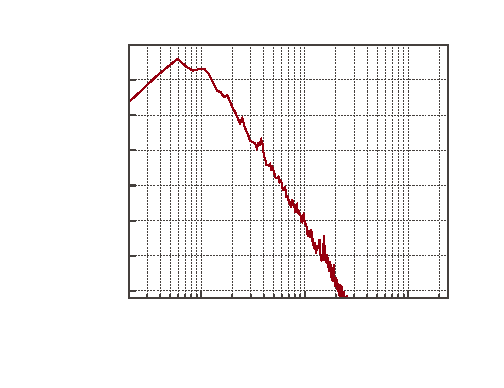
\includegraphics{Images/plot}}%
    \gplfronttext
  \end{picture}%
\endgroup

		\caption{LFE channel frequency spectrum}
	\end{figure}
\end{frame}

\subsection{Tables}
\begin{frame}{Table}
\begin{table}[]
	\caption{Selection of window function and their properties}
	\begin{tabular}[]{lrrr}
		\toprule
		\textbf{Window}			& \multicolumn{1}{c}{\textbf{First side lobe}}	
		                    & \multicolumn{1}{c}{\textbf{3\,dB bandwidth}}
		                    & \multicolumn{1}{c}{\textbf{Roll-off}} \\
		\midrule
		Rectangular				& 13.2\,dB	& 0.886\,Hz/bin	& 6\,dB/oct		\\[0.25em]
		Triangular				& 26.4\,dB	& 1.276\,Hz/bin	& 12\,dB/oct	\\[0.25em]
		Hann					& 31.0\,dB	& 1.442\,Hz/bin	& 18\,dB/oct	\\[0.25em]
		Hamming					& 41.0\,dB	& 1.300\,Hz/bin	& 6\,dB/oct		\\
		\bottomrule
	\end{tabular}
	\label{tab:WindowFunctions}
\end{table}
\end{frame}

\subsection{Formulas}
\begin{frame}{Formulas}
\begin{block}{Fourier Integral}
\begin{equation*}
F(\textrm{j}\omega) = \int\limits_{-\infty}^{\infty} f(t)\cdot\textrm{e}^{-\textrm{j}\omega t} dt
\end{equation*}
\end{block}
\begin{block}{Factorial}
\begin{equation*}
	n! = 1\cdot 2 \cdot 3 \cdot\ldots\cdot n = \prod_{k=1}^n k
\end{equation*}
\end{block}
\end{frame}

\begin{frame}{Mindmap with TikZ}
\centering
\resizebox{\textheight}{!}{%
\begin{tikzpicture}[scale=0.88]
	%\tikzset{every child/.append style={level distance=250}}
	\path[mindmap,concept color=sleekSec1Comp,text=sleekWarmGreyDark,yshift=3cm]
	node[concept] {\TeX}
	[clockwise from=-30]
	child[concept color=sleekSec2Dark,text=white] { node[concept] {\textcolor{white}{XeTeX}} }
	child[concept color=sleekSec1CompDark,text=white,yshift=0.1cm] { node[concept]{ConTex} }
	child[concept color=sleekSec1Dark,text=white] { node[concept] {\LaTeX} };
\end{tikzpicture}%
}
\end{frame}

\subsection{Footnote}
\begin{frame}{Footnotes}
	Lorem ipsum dolor sit amet, consetetur sadipscing elitr, sed diam nonumy eirmod tempor invidunt ut labore et dolore magna aliquyam erat, sed diam voluptua. At vero eos et accusam et justo duo dolores et ea rebum. Stet clita kasd gubergren, no sea takimata sanctus est Lorem ipsum dolor sit amet. Lorem \footnote{Lorem ipsum dolor sit amet} ipsum dolor sit amet, consetetur sadipscing elitr, sed diam nonumy eirmod tempor invidunt ut labore et dolore magna aliquyam erat, sed diam voluptua. At vero eos et accusam et justo duo dolores et ea rebum. Stet clita kasd gubergren, no sea takimata sanctus est Lorem ipsum dolor sit amet.
\end{frame}

\subsection{Notes}
\begin{frame}{slide with associated notes slide}
    This slide is for the audience.

	The following programmes are suitable for its presentation:
	\begin{itemize}
		\item Splitshow (Mac OS X)\\url{https://code.google.com/p/splitshow/}
		\item pdf-presenter (Windows)\\url{https://code.google.com/p/pdf-presenter/}
	\end{itemize}
\end{frame}

\note{
    Use this slide for your notes on the presentation.
    
	The following programmes are suitable for your presentation:
	\begin{itemize}
		\item Splitshow (Mac OS X)\\\url{https://code.google.com/p/splitshow/}
		\item pdf-presenter (Windows)\\\url{https://code.google.com/p/pdf-presenter/}
	\end{itemize} 
}

\subsection{Columns}
\begin{frame}{Two columns}
	\begin{multicols}{2}
		Lorem ipsum dolor sit amet, consetetur sadipscing elitr, sed diam nonumy eirmod tempor invidunt ut labore et dolore magna aliquyam erat, sed diam voluptua. At vero eos et accusam et justo duo dolores et ea rebum. Stet clita kasd gubergren, no sea takimata sanctus est Lorem ipsum dolor sit amet.
		\begin{itemize}
        	\item one entry
        	\item another entry
		\end{itemize}
	\end{multicols}
\end{frame}

\begin{frame}{Column break}
	\begin{multicols}{2}
		Lorem ipsum dolor sit amet, consetetur sadipscing elitr, sed diam nonumy eirmod tempor invidunt ut labore et dolore magna aliquyam erat, sed diam voluptua. At vero eos et accusam et justo duo dolores et ea rebum. Stet clita kasd gubergren, no sea takimata sanctus est Lorem ipsum dolor sit amet.
		\columnbreak
		\begin{itemize}
        	\item one entry
        	\item another entry
		\end{itemize}
	\end{multicols}
\end{frame}

\begin{frame}{References}
	\begin{thebibliography}{10}
    
	\beamertemplatebookbibitems
	\bibitem{Oppenheim2009}
	Alan~V.~Oppenheim
	\newblock \doublequoted{Discrete-Time Signal Processing}
	\newblock Prentice Hall Press, 2009

	\beamertemplatearticlebibitems
	\bibitem{EBU2011}
	European~Broadcasting~Union
	\newblock \doublequoted{Specification of the Broadcast Wave Format (BWF)}
	\newblock 2011
  \end{thebibliography}
\end{frame}

\section{Outlook}
\begin{frame}{To do}
	\begin{itemize}
		\item An option to a more complete footline needs to be added.
	\end{itemize}
\end{frame}

\begin{frame}{Questions, Comments, Contact}
	The SLEEK theme is licensed under the \quoted{GNU Public License}. So it may be redistributed and modified as long as the license type is kept.
	
	Please feel free to contact me if you have any questions or comments.
	\begin{itemize}
		\item \href{mailto:up201806093@up.pt}{up201806093@up.pt}
	\end{itemize}
\end{frame}

\end{document}






